\subsection{Connected Data Across Views \href{http://randy.cs.columbia.edu/lineage/pgbench-connect/pgbench.html}{(\underline{link})}}\label{connect}
\begin{figure}[H]
	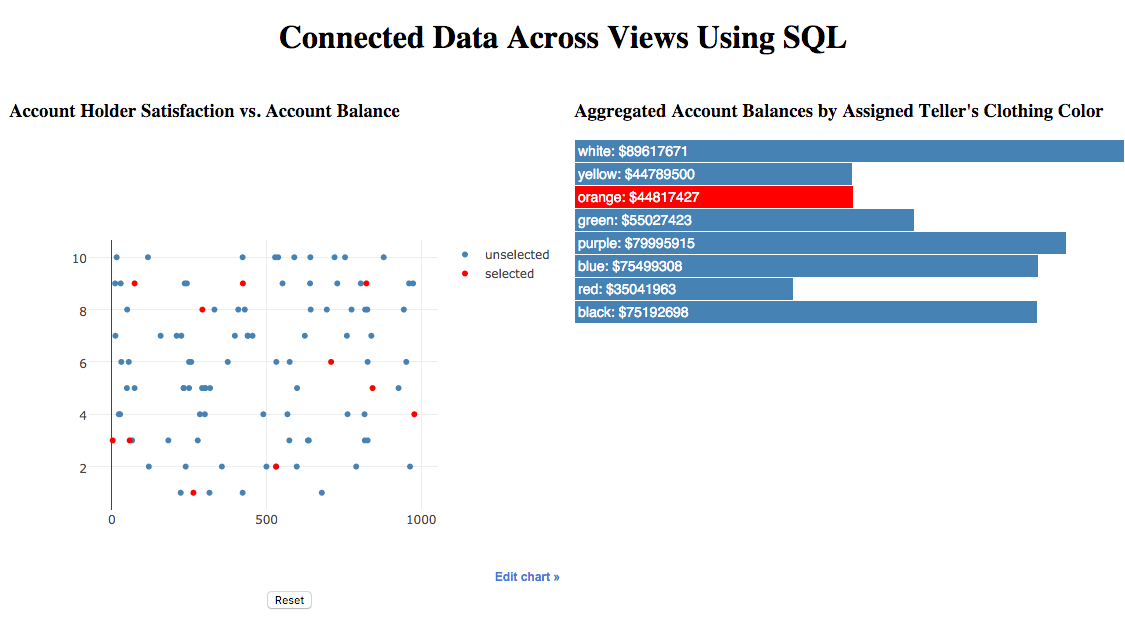
\includegraphics[width=\columnwidth]{figures/connect}
	\caption{A screenshot of the visualizations described in \autoref{connect}
	}
	\label{fig_connect}
\end{figure}
\subsubsection{Vega}
\subsubsection*{Scatter Plot ($V_1$, left view in Figure~\ref{fig_connect})}
\lstinputlisting[language=json, tabsize=2, emptylines=0]{../pgbench-connect/vega/scatterplot.json}
\subsubsection*{Bar Chart ($V_2$, right view in Figure~\ref{fig_connect})}
\lstinputlisting[language=json, tabsize=2, emptylines=0]{../pgbench-connect/vega/barchart.json}
\subsubsection{Succinct Event-driven Description (SED) \#1 (whiteboarded on 11/12)}
Let $V_1$ be the scatter plot.
Let $V_2$ be the bar chart.
\begin{align*}
	V_1&= \mathlarger{\pi}_{circle}(\bf{accounts})\\
	S_1&= \mathlarger{\pi}_{circle}(\mathlarger{\sigma}_{P_1}(\bf{accounts}))\\
	V_2&= \mathlarger{\pi}_{rect}(\mathlarger{\gamma}_{ccolor, \text{SUM}(abalance)}(\bf{accounts}\bowtie{}\bf{tellers}))\\
	S_2&= \mathlarger{\pi}_{rect}(\mathlarger{\gamma}_{ccolor, \text{SUM}(abalance)}(\mathlarger{\sigma}_{P_2}(\bf{accounts}\bowtie{}\bf{tellers})))\\
	init()&:\\
	reset()&:\\
	&: P_1 = P_2 = *\\
	&: S_1.color = S_2.color = \texttt{steelblue}\\
	click(V_2)&:\\
	&: P_2 = ``\text{WHERE}~ccolor=click.ccolor"\\
	&: P_1 = ``\text{WHERE}~aid~\text{IN~lineage}(S_2, \bf{accounts})"\\
	&: S_1.color = S_2.color = \texttt{red}\\
\end{align*}
\subsubsection{SED \#2}
The same interaction can be described using a single predicate for both views.
\begin{align*}
	V_1&= \mathlarger{\pi}_{circle}(\bf{accounts})\\
	S_1&= \mathlarger{\pi}_{circle}(\mathlarger{\sigma}_{P_2}(\bf{accounts}\bowtie{}\bf{tellers})))\\
	V_2&= \mathlarger{\pi}_{rect}(\mathlarger{\gamma}_{ccolor, \text{SUM}(abalance)}(\bf{accounts}\bowtie{}\bf{tellers}))\\
	S_2&= \mathlarger{\pi}_{rect}(\mathlarger{\gamma}_{ccolor, \text{SUM}(abalance)}(\mathlarger{\sigma}_{P_2}(\bf{accounts}\bowtie{}\bf{tellers})))\\
	init()&:\\
	reset()&:\\
	&: P_2 = *\\
	&: S_1.color = S_2.color = \texttt{steelblue}\\
	click(V_2)&:\\
	&: P_2 = ``\text{WHERE}~ccolor=click.ccolor"\\
	&: S_1.color = S_2.color = \texttt{red}\\
\end{align*}
\subsubsection{SED \#3 (expanded to include clicks on $V_1$)}\label{connect_3}
\begin{align*}
	V_1&= \mathlarger{\pi}_{circle}(\bf{accounts})\\
	S_1&= \mathlarger{\pi}_{circle}(\mathlarger{\sigma}_{P_1}(\bf{accounts}))\\
	V_2&= \mathlarger{\pi}_{rect}(\mathlarger{\gamma}_{ccolor, \text{SUM}(abalance)}(\bf{accounts}\bowtie{}\bf{tellers}))\\
	S_2&= \mathlarger{\pi}_{rect}(\mathlarger{\gamma}_{ccolor, \text{SUM}(abalance)}(\\&\mathlarger{\sigma}_{P_2}(\bf{accounts}\bowtie{}\bf{tellers})))\\
	init()&:\\
	reset()&:\\
	&: P_1 = P_2 = *\\
	&: S_1.color = S_2.color = \texttt{steelblue}\\
	select(V_1)&:\\
	&: reset()\\
	&: P_1 = ``\text{WHERE}~aid~\text{IN}~\mathlarger{\pi}_{\bf{accounts}}(select)"\\
	&: P_2 = ``\text{WHERE}~ccolor\text{IN~SELECT~DISTINCT}~ccolor~\\&\text{FROM}~\mathlarger{\pi}_{\bf{accounts}}(S_1)\bowtie{}\bf{tellers}"\\
	&: S_1.color = S_2.color = \texttt{red}\\
	click(V_2)&:\\
	&: reset()\\
	&: P_2 = ``\text{WHERE}~ccolor=click.ccolor"\\
	&: P_1 = ``\text{WHERE}~aid~\text{IN~lineage}(S_2, \bf{accounts})"\\
	&: S_1.color = S_2.color = \texttt{red}\\
\end{align*}
\subsection{Aggregation Filtering \href{http://randy.cs.columbia.edu/lineage/pgbench-filter/pgbench.html}{(\underline{link})}}\label{filter}
\begin{figure}[H]
	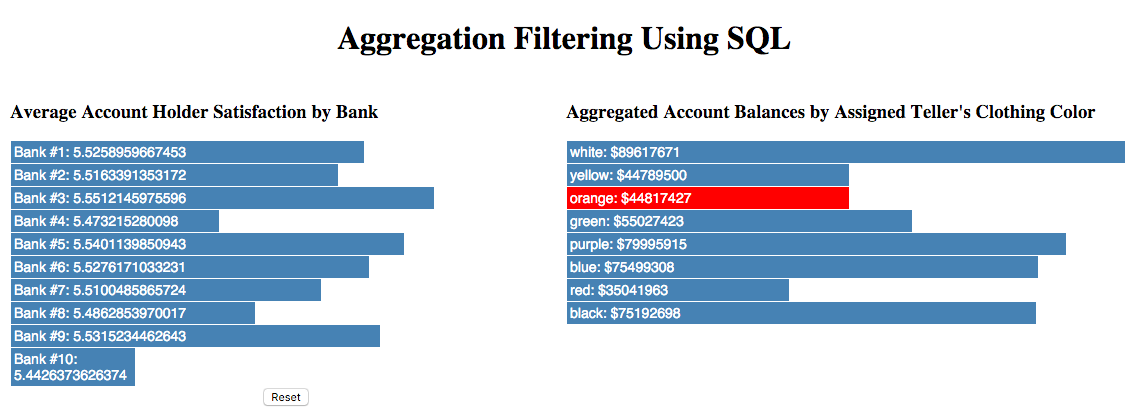
\includegraphics[width=\columnwidth]{figures/filter}
	\caption{A screenshot of the visualizations described in \autoref{filter}
	}
	\label{fig_filter}
\end{figure}
\subsubsection{Vega}
\subsubsection*{Satisfaction Bar Chart ($V_3$, left view in Figure~\ref{fig_filter})}
\lstinputlisting[language=json, tabsize=2, emptylines=0]{../pgbench-filter/vega/satisfactionbars.json}
\subsubsection*{Balance Bar Chart ($V_4$, right view in Figure~\ref{fig_filter})}
\lstinputlisting[language=json, tabsize=2, emptylines=0]{../pgbench-filter/vega/balancebars.json}
\subsubsection{SED}
Let $V_3$ be the satisfaction bar chart.
Let $V_4$ be the balance bar chart.
\begin{align*}
	V_3&= \mathlarger{\pi}_{rect}(\mathlarger{\gamma}_{bid, \text{AVG}(satisfaction)}(\bf{accounts}\bowtie{}\bf{tellers}))\\
	S_3&= \mathlarger{\pi}_{rect}(\mathlarger{\gamma}_{bid, \text{AVG}(satisfaction)}(\mathlarger{\sigma}_{P_3}(\bf{accounts}\bowtie{}\bf{tellers})))\\
	V_4&= \mathlarger{\pi}_{rect}(\mathlarger{\gamma}_{ccolor, \text{SUM}(abalance)}(\bf{accounts}\bowtie{}\bf{tellers}))\\
	S_4&= \mathlarger{\pi}_{rect}(\mathlarger{\gamma}_{ccolor, \text{SUM}(abalance)}(\mathlarger{\sigma}_{P_4}(\bf{accounts}\bowtie{}\bf{tellers})))\\
	init()&:\\
	reset()&:\\
	&: P_3 = P_4 = *\\
	&: S_3.color = S_4.color = \texttt{steelblue}\\
	click(V_4)&:\\
	&: P_3 = P_4 = ``\text{WHERE}~ccolor=click.ccolor"\\
	&: S_3.color = S_4.color = \texttt{red}\\
\end{align*}
\subsection{Filter \& Elaborate}\label{elaborate}
\begin{figure}[H]
	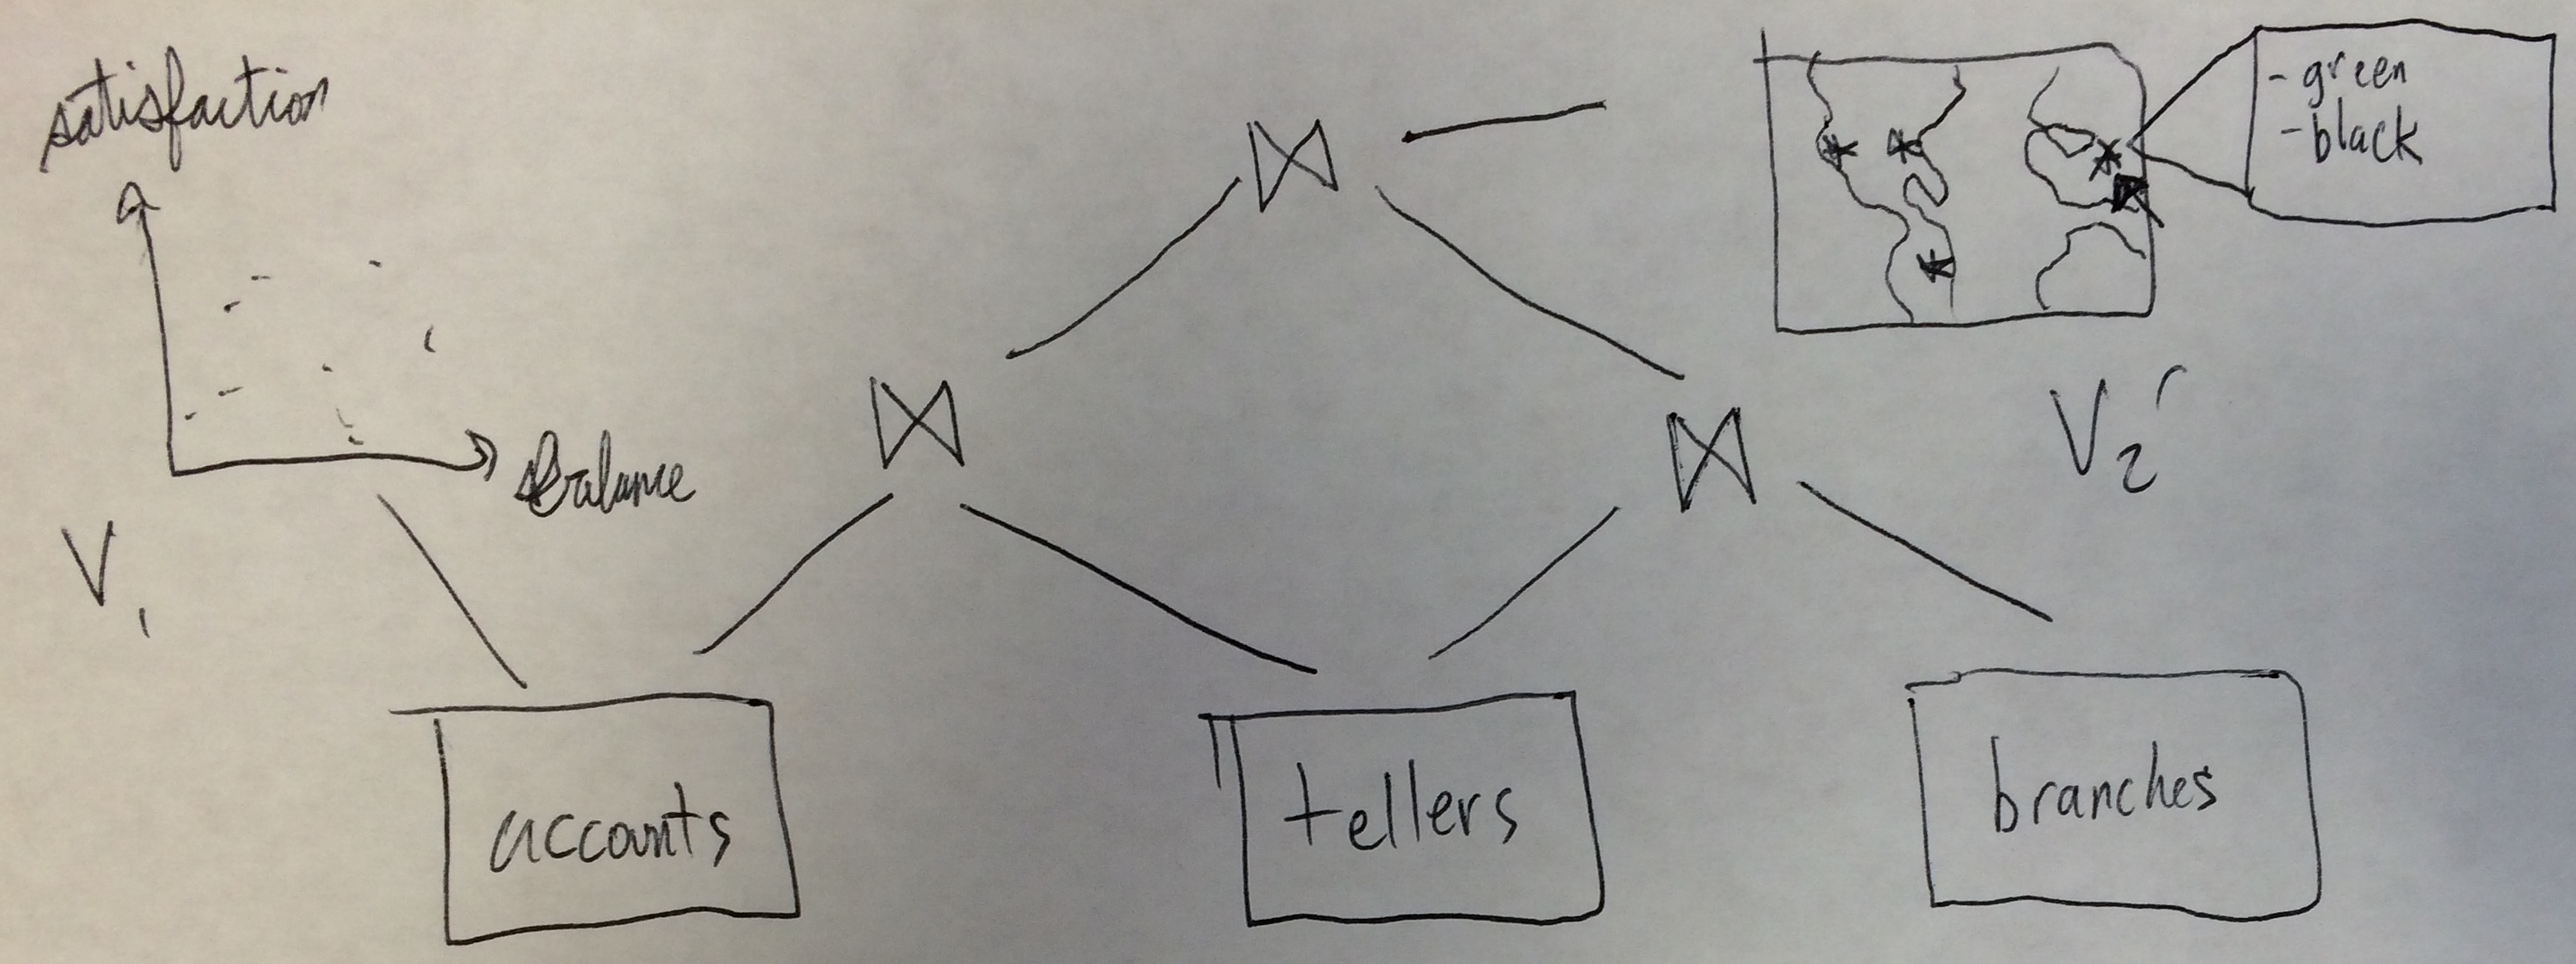
\includegraphics[width=\columnwidth]{figures/elaborate}
	\caption{A cartoon of the visualizations described in \autoref{elaborate}
	}
	\label{fig_elaborate}
\end{figure}
Consider an amendment to the visualization in \autoref{connect_3} wherein the bar chart $V_2$ is replaced by a map showing the branch locations $V_2'$.
On mousing over any of the branch locations, all colors worn by any of the tellers at that branch are shown in a flyout.
When some accounts are selected from the scatterplot, only the tellers who manage those accounts are considered.
\subsubsection{SED \#1}
Let $V_1$ be the scatter plot.
Let $V_2'$ be the map.
\begin{align*}
	V_1&= \mathlarger{\pi}_{circle}(\bf{accounts})\\
	S_1&= \mathlarger{\pi}_{circle}(\mathlarger{\sigma}_{P_1}(\bf{accounts}))\\
	V_2'&= \mathlarger{\pi}_{star}(\mathlarger{\gamma}_{ccolor, \text{SUM}(abalance)}(\bf{accounts}\bowtie{}\bf{tellers}))\\
	S_2'&= \mathlarger{\pi}_{ccolor}(\mathlarger{\sigma}_{P_2'}(\bf{accounts}\bowtie{}\bf{tellers}\bowtie{}\bf{branches}))\\
	init()&:\\
	reset()&:\\
	&: P_1 = *\\
	&: S_1.color = \texttt{steelblue}\\
	select(V_1)&:\\
	&: reset()\\
	&: P_1 = ``\text{WHERE}~aid~\text{IN}~\mathlarger{\pi}_{\bf{accounts}}(select)"\\
	&: S_1.color = \texttt{red}\\
	mouseover(V_2)&:\\
	&: P_2' = ``\text{WHERE}~aid~\text{IN}~\mathlarger{\pi}_{\bf{accounts}}(S_1)~\text{AND}\\&bid=\mathlarger{\pi}_{\bf{branches.bid}}(mouseover.star)"\\
	&: pointer.flyout = \mathlarger{\pi}_{textbox}(S_2')\\
	&: pointer.flyout.visible = \texttt{true}\\
	mouseoff(V_2)&:\\
	&: pointer.flyout.visible = \texttt{false}\\
\end{align*}
\subsubsection{SED \#2 (holistic aggregation)}
Consider a variant of this same visualization with a more complicated aggregation function.
Namely, the flyout now shows only the most frequently-worn color for the given bank (considering only tellers who manage the selected accounts in $V_1$).
The complexity of the aggregation function does not affect the applicability of data cubes - only the amount of computation necessary to compute them.
\begin{align*}
	V_1&= \mathlarger{\pi}_{circle}(\bf{accounts})\\
	S_1&= \mathlarger{\pi}_{circle}(\mathlarger{\sigma}_{P_1}(\bf{accounts}))\\
	V_2'&= \mathlarger{\pi}_{star}(\mathlarger{\gamma}_{ccolor, \text{SUM}(abalance)}(\\&\bf{accounts}\bowtie{}\bf{tellers}))\\
	S_2'&= \mathlarger{\gamma}_{\text{MostFrequent}(ccolor)}(\mathlarger{\sigma}_{P_2'}(\\&\bf{accounts}\bowtie{}\bf{tellers}\bowtie{}\bf{branches}))\\
	init()&:\\
	reset()&:\\
	&: P_1 = *\\
	&: S_1.color = \texttt{steelblue}\\
	select(V_1)&:\\
	&: reset()\\
	&: P_1 = ``\text{WHERE}~aid~\text{IN}~\mathlarger{\pi}_{\bf{accounts}}(select)"\\
	&: S_1.color = \texttt{red}\\
	mouseover(V_2)&:\\
	&: P_2' = ``\text{WHERE}~aid~\text{IN}~\mathlarger{\pi}_{\bf{accounts}}(S_1)~\text{AND}\\&bid=\mathlarger{\pi}_{\bf{branches.bid}}(mouseover.star)"\\
	&: pointer.flyout = \mathlarger{\pi}_{textbox}(S_2')\\
	&: pointer.flyout.visible = \texttt{true}\\
	mouseoff(V_2)&:\\
	&: pointer.flyout.visible = \texttt{false}\\
\end{align*}
\subsection{Connect (multiple tellers per account)}\label{sparse}
\begin{figure}[H]
	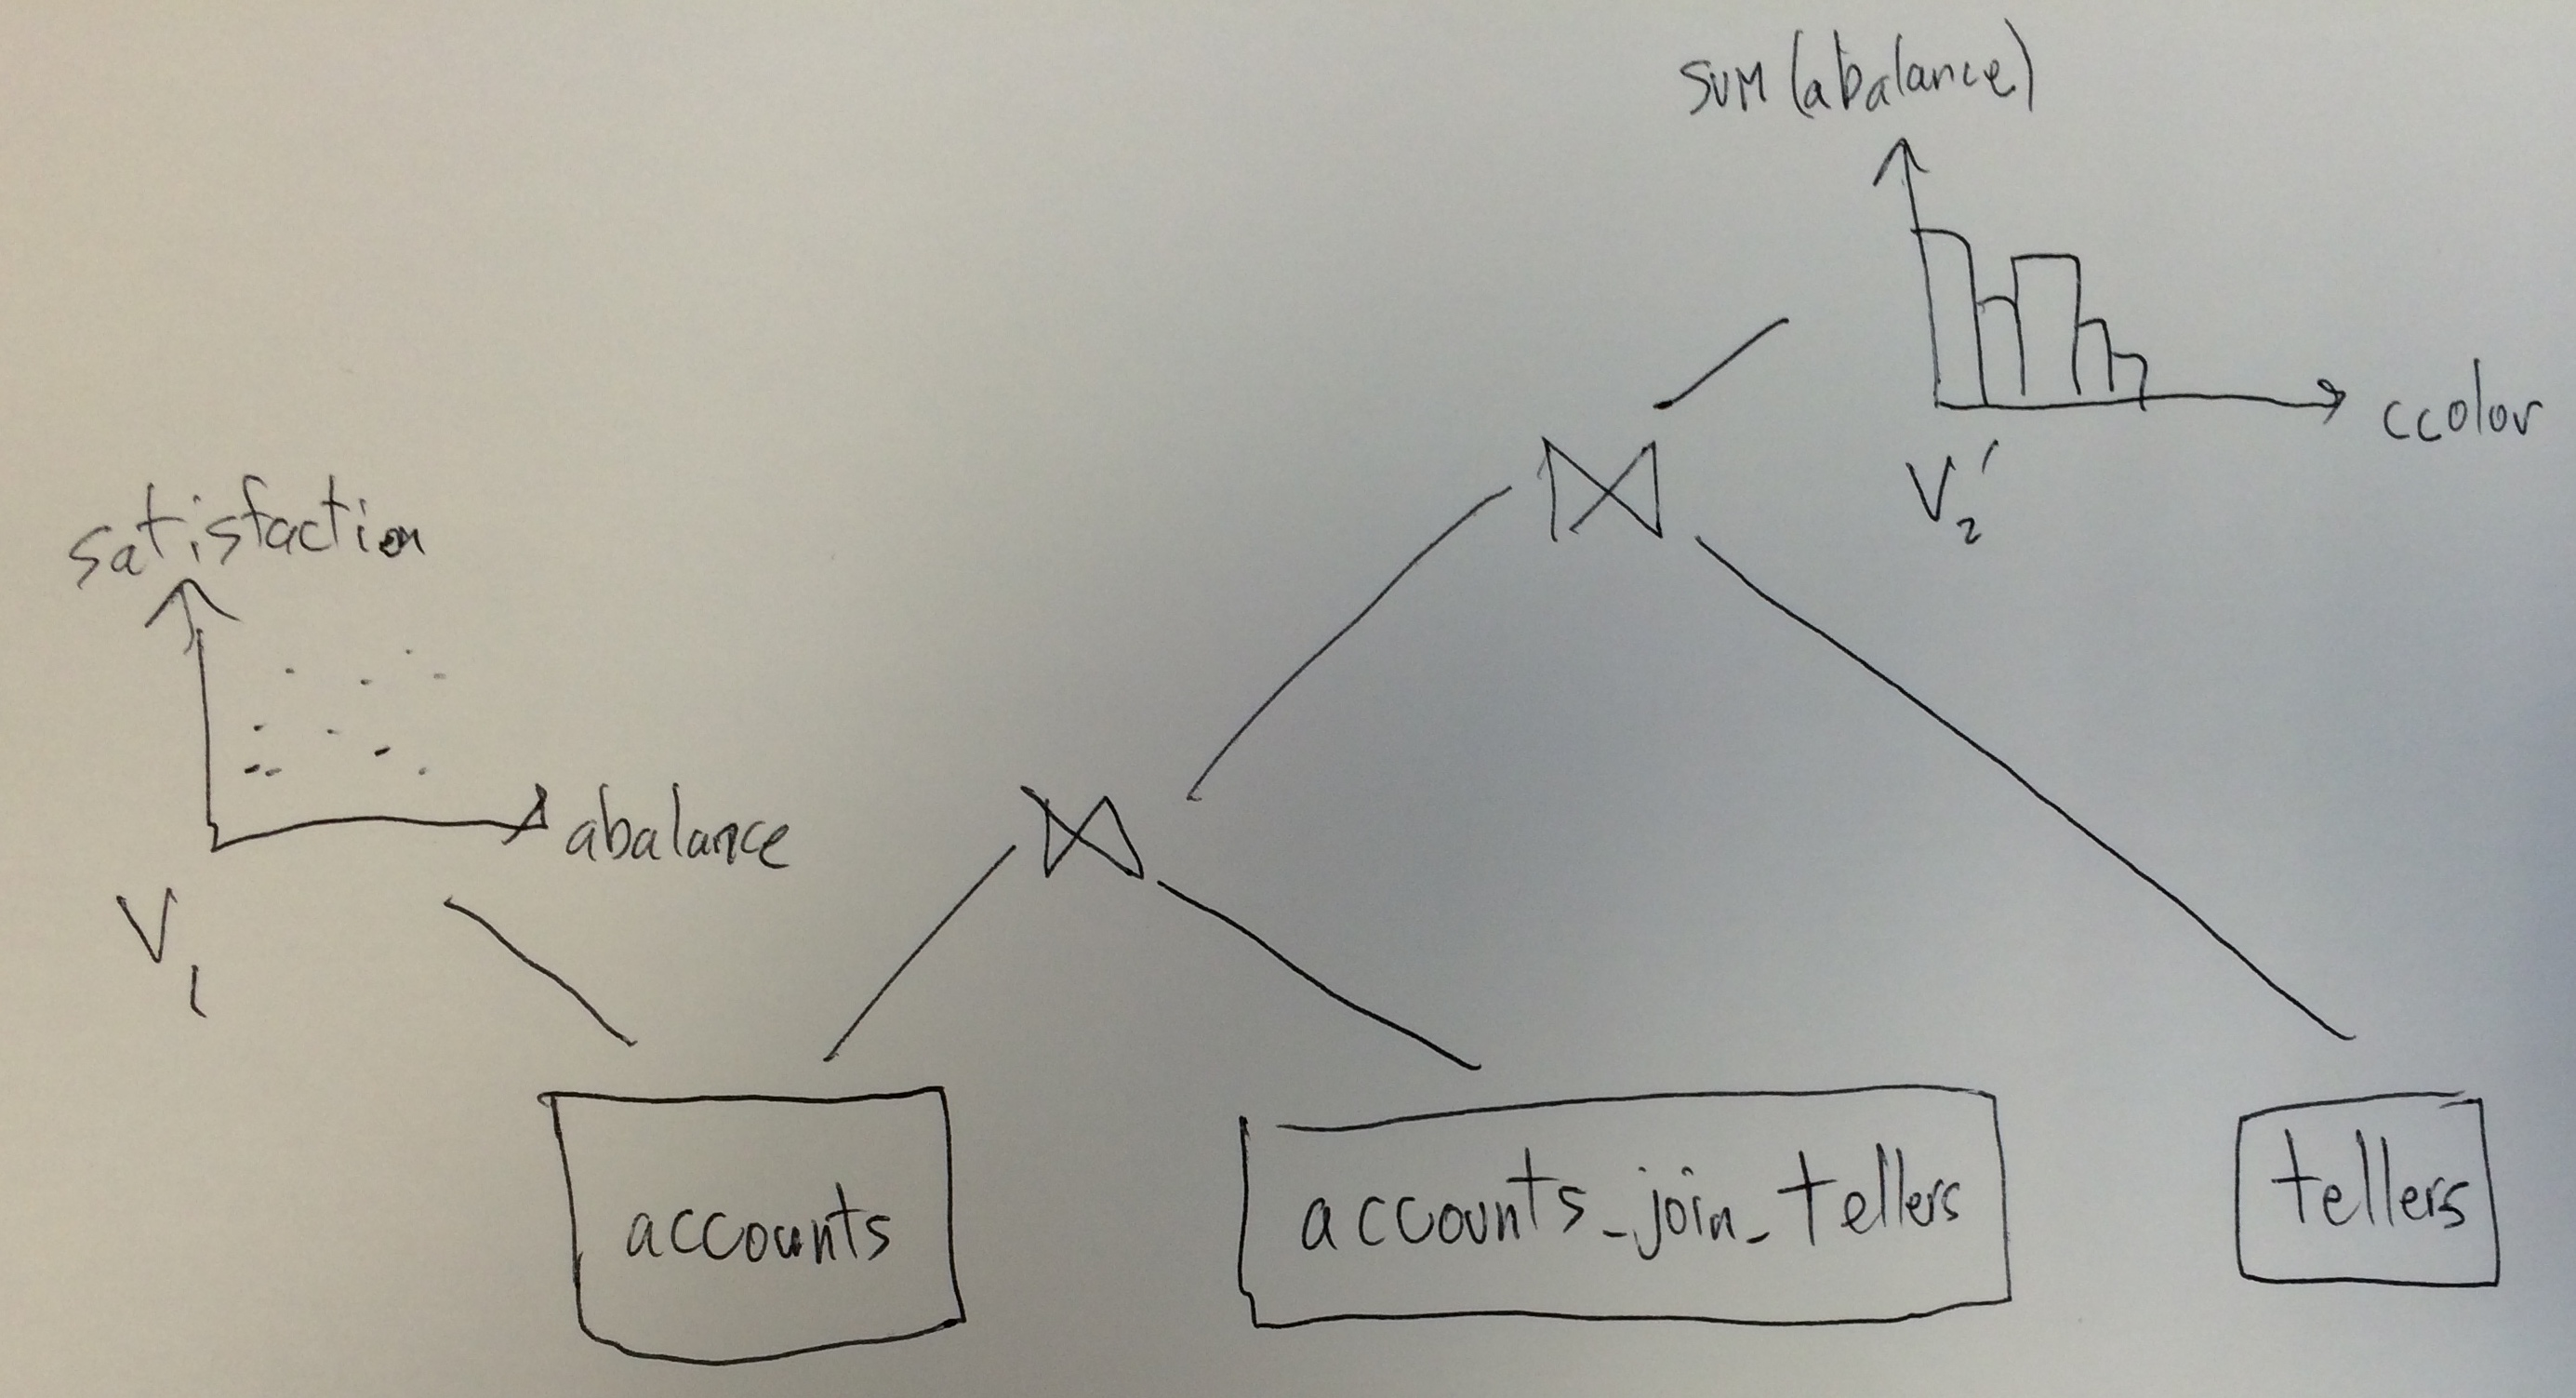
\includegraphics[width=\columnwidth]{figures/sparse}
	\caption{A cartoon of the visualizations described in \autoref{sparse}
	}
	\label{fig_sparse}
\end{figure}
Consider an amendment to the visualization in \autoref{connect_3} wherein each account is managed by two tellers.
In order to associate account records with teller records, a join table named \textbf{accounts\_join\_tellers} is used.
This interaction can be indexed with a data cube just as in \autoref{connect_3}.
\subsubsection{SED}
\begin{align*}
	V_1&= \mathlarger{\pi}_{circle}(\bf{accounts})\\
	S_1&= \mathlarger{\pi}_{circle}(\mathlarger{\sigma}_{P_1}(\bf{accounts}))\\
	V_2&= \mathlarger{\pi}_{rect}(\mathlarger{\gamma}_{ccolor, \text{SUM}(abalance)}(\\&\bf{accounts}\bowtie{}\bf{accounts\_join\_tellers}\bowtie{}\bf{tellers}))\\
	S_2&= \mathlarger{\pi}_{rect}(\mathlarger{\gamma}_{ccolor, \text{SUM}(abalance)}(\\&\mathlarger{\sigma}_{P_2}(\bf{accounts}\bowtie{}\bf{accounts\_join\_tellers}\bowtie{}\bf{tellers})))\\
	init()&:\\
	reset()&:\\
	&: P_1 = P_2 = *\\
	&: S_1.color = S_2.color = \texttt{steelblue}\\
	select(V_1)&:\\
	&: reset()\\
	&: P_1 = ``\text{WHERE}~aid~\text{IN}~\mathlarger{\pi}_{\bf{accounts}}(select)"\\
	&: P_2 = ``\text{WHERE}~ccolor\text{IN~SELECT~DISTINCT}~ccolor~\\&\text{FROM}~\mathlarger{\pi}_{\bf{accounts}}(S_1)\bowtie{}\bf{accounts\_join\_tellers}\bowtie{}\bf{tellers}"\\
	&: S_1.color = S_2.color = \texttt{red}\\
	click(V_2)&:\\
	&: reset()\\
	&: P_2 = ``\text{WHERE}~ccolor=click.ccolor"\\
	&: P_1 = ``\text{WHERE}~aid~\text{IN~lineage}(S_2, \bf{accounts})"\\
	&: S_1.color = S_2.color = \texttt{red}\\
\end{align*}
\subsection{Vega vs. Alternatives}
\underline{Similarities}:
\begin{enumerate}
	\item Both descriptions are partially declarative and partially stateful.
	\item Both descriptions are event-driven, with state changes propagating up from interaction events to modify intermediate state, and eventually the rendered views (if necessary).
	\item The tables involved in rendering each view are immediately apparent from the description of the view/marks.
\end{enumerate}
\underline{Differences}:
\begin{enumerate}
	\item The alternate description is far more succinct than Vega.
	\item The alternate description leaves out many details.
		For example:
		\begin{itemize}
			\item scaling and position details contained in the projections $\mathlarger{\pi}_{circle}$ and $\mathlarger{\pi}_{rect}$;
			\item descriptive names for scales, predicates, and marks; and
			\item scaling, position, and signal details corresponding to interaction events (this makes it difficult to specify predicates which depend on those events).
		\end{itemize}
\end{enumerate}
% \subsection{Possible Indicators That Lineage Can Be Used for Optimization}
% \begin{enumerate}
% 	\item The same tables are seen in the definitions for two different selection symbols.
% 	\item The predicate used to define one selection symbol contains another selection symbol.
% 	\item Two selection symbols use the same predicate.
% \end{enumerate}
% \subsection{Possible Indicators That Data Cubes Can Be Used for Optimization}
% \begin{enumerate}
% 	\item The same exact mappings of the same tables are seen in the definitions for two different selection symbols.
% \end{enumerate}
\subsection{Possible Cases Where Data Cubes CanNOT Be Used for Optimization}
\begin{enumerate}
	\item Different aggregations are used in the different views $\Rightarrow$ \textbf{Rejected} (both aggregations can be stored in each cell, and each superaggregate)
	\item Using a holistic aggregate $\Rightarrow$ \textbf{Rejected} (the data cube can still hold the aggregate and superaggregate values; they will just take longer to compute)
	\item Loading new data dynamically $\Rightarrow$ \textbf{Undecided}
	\item It is impractical to calculate the full data cube, and aggregations must be done dynamically depending on interactions $\Rightarrow$ \textbf{Probably!}
\end{enumerate}
\subsection{Possible Uses of Indexed Data Lineage in Interactions}
\begin{enumerate}
	\item To decide what filter to apply to a data cube.
		\begin{itemize}
			\item Scenario: A viz spec describes how $V_1$ is related to the data, how $V_2$ is related to the data, and how $V_2$ changes with selections on $V_1$ from a set of options (e.g. ``connected" - related marks are highlighted in $V_2$, or ``filtered" - unrelated marks are removed from $V_2$).
			Now the programmer does not need to specify the predicate for filtering the data cube.
			The predicate is provided by the lineage of the selection in $V_1$.
			\item Usefulness Criteria:
				\begin{enumerate}
					\item Calculating the lineage is computationally intensive.
					\item Determining the data cube filter is otherwise logically complex or difficult to describe.
				\end{enumerate}
		\end{itemize}
	\item To decide (immediately) which data tile(s) are needed.
	\item To decide which attributes/dimensions need to be included in the data cube.
\end{enumerate}